\documentclass{article}
\usepackage{graphicx}
\usepackage{wrapfig}
\usepackage{amsmath}
\usepackage{subcaption}
\usepackage[margin=1.0in]{geometry}
\usepackage{lineno}
\linenumbers
\linespread{2}
\renewcommand\linenumberfont{\normalfont\bfseries\small}

\begin{document}
\section{Experiment}
Anion photoelectron spectroscopy (APES) measurements from 1996 indicate that the low-lying states of the CuO molecule are composed of 3d9 and 3d10 states [ref 48.pdf]. Shown below are the most recent APES measurements for the CuO molecule, all state assignments except for the $b^4\Sigma$ state have been verified by other experiments.

\begin{wrapfigure}{r}{0.4\textwidth}
  \begin{center}
    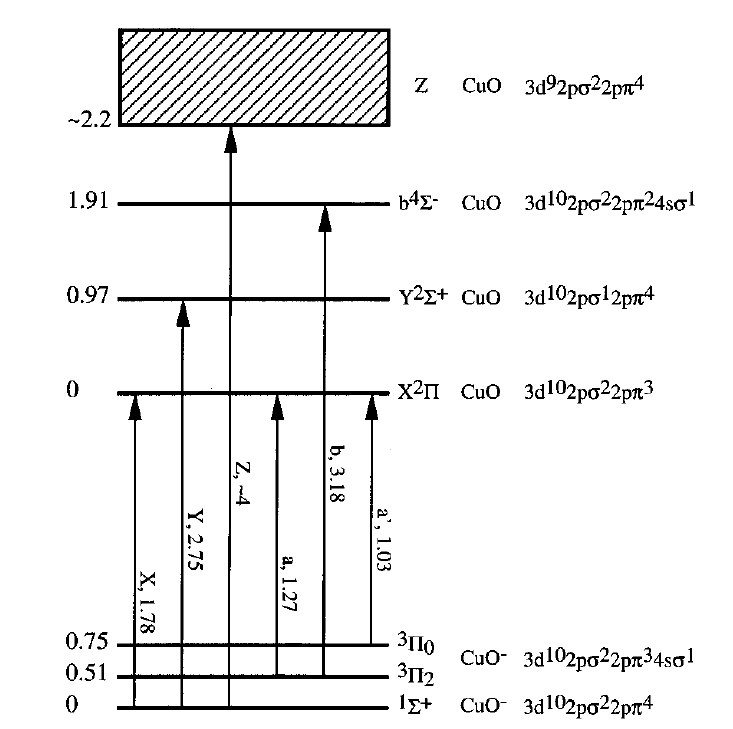
\includegraphics[width=0.3\textwidth]{APES.png}
  \end{center}
  \caption{APES measurements on CuO molecule.}
\end{wrapfigure}

The APES measurements yield a ground state of CuO is $X^2\Pi$ and the first excited state $Y^2\Sigma^+$, which are consistent with higher resolution PES measurements and various other theoretical and experimental measurements [multiple ref]. The $X^2\Pi \rightarrow Y^2\Sigma^+$ excitation corresponds to an excitation $O p_\sigma \rightarrow O p_\pi$, and has a measured energy of 0.97 eV. The APES measurements also find a block of excitations starting at 2.20 eV which correspond to the 3d9 excited states of CuO. Earlier measurements have found similar results. Further, both these APES measurements and Laser Induced Flourescence measurements in 1980 [ref] have found a quartet state at 1.91 eV. This state has been assigned as $^4\Sigma$, but the argumentation for its assignment is based on an assumption that the quartet state measured in APES is the lowest possible energy quartet state. 

Further, since the lowest energy states of the CuO molecule are 3d104s0, 3d94s0 and 3d94s1 in character, it is instructive to look at experimental measurements of the properties of the Cu$^+$ and Cu$^{2+}$ ions [ref]. The Cu$^{2+}$ ion has a ground state of character 3d94s0, and a first excited state around 6.7 eV of 3d84s1, indicating that the 3d8 sector of eigenstates may be ignored in our study. The Cu$^+$ ion has a ground state character of 3d10, and two excited states at 2.72 and 3.26 eV of character 3d94s1. These two low energy excited states differ in their total spin, the lower energy state being a $^3D$ state and the higher energy state being a $^1D$ state. This indicates to us that there is a Hund's coupling on the copper atom of $J_H = -0.54 eV$.

\section{Sampling scheme}
In order to do DMD we need to densely sample the low energy space (LES). In our case, we will define the LES as the span of a set of base states. Since we know that our system has a low energy 3d9 and 3d10 sector, we will consider base states with either 9 or 10 electrons in the d-orbitals. Further, in order to consider the effects of a possible Hund's coupling arising in our effective theory from the Cu atom $J_H$, we will need to consider states with both $S_z=1/2, 3/2$. When moving to QMC, we will not be able to consider linear combinations of states with different $S_z$, so in order to sample the effect of $J_H$ densely, we would also like to consider "spin-flip partner" states in the $S_z=1/2$ sector. Consider for example a state Cu3d9\! 4s1 O2p$_{\pi}$3 in the $S_z=1/2$ sector. The half-filled orbitals can have electrons with configuration $up\ up\ dn$ or $up\ dn\ up$, the prior which would have a Hund's descriptor $\frac{1}{2}$ and the latter $-\frac{1}{2}$. Further, we would like to use single determinant Slater-Jastrow wave functions since they have proven to be quite accurate trial wave functions on previous QMC calculations for transition metal oxide molecules [ref]. In order to meet all of these considerations, we chose to collect base states by using spin and spatial-symmetry targeted unrestricted Kohn Sham (UKS) [ref] single determinant states using a B3LYP functional [ref] and Trail-Needs basis with the corresponding pseudopotentials [ref]. 

First, we generated all the unique base states in the 3d9 and 3d10 sectors using this method. In order to sample the span of the base states we used a shell sampling technique which samples in shells of fixed radius around each of the base states using base state weights of 0.1 - 1.0 in increments of 0.1. Our final set of states in our span were then multiplied by a three-body Jastrow factor, which was optimized on the UKS ground state. Fixed node Diffusion Monte Carlo (FN-DMC) [ref] calculations were run with these states as trial wave functions with a timestep of 0.01 and Tmoves [ref]  in order to get 1-/2-density matrix elements and total energies.

\section{RDM basis}
There were two choices of the RDM basis that we could have used, either an IAO basis or an MO basis. The IAO basis is more theoretically pleasing because it's a set of functions which best capture the variation between the the Cu 3d, O 2p, and Cu 4s orbitals from our different base states. Further, the IAO basis is beneficial for representing local interactions since they are localized orbitals. However, the IAO basis has the drawback that many 1-body parameters will be correlated, for example $n_{p_\pi}$ and $t_\pi$. The MO basis choice is more arbitrary since we don't know a way of constructing "intrinsic molecular orbitals," but the RDM elements in this basis tend to vary in a less correlated fashion. This is because, to lowest order, excitations of CuO look very similar to single-particle molecular orbital excitations, so variations in the MO descriptor space are nearly orthogonal. In order to take advantage of the benefits of both bases, I chose to do my model fitting using a mixture of both bases: an MO basis for the non-interacting parts (n, t) and an IAO basis for the interacting pieces (J, U, etc.). In the end we can rotate the MO parameters into the IAO basis, leading to a fully localized representation of our model. The IAO basis I used was constructed on the collection of active MOs (Cu 3d, O 2p and Cu 4s) from every base state. The MO basis selected was the the set of active MOs from the first excited ROKS state of CuO. This is because the single-Slater determinant ground state of CuO from ROKS breaks O$p_x, p_y$ and Cu$d_{xz}, d_{yz}$ degeneracies. These degeneracies are restored in the first excited state ROKS calculation. Later in the analysis, a weighted linear regression (WLS) is used to fit our model, and it will be shown that the WLS assigns nearly zero weight to any sampled states which have a 1-rdm trace far less than 15, the total number of electrons expected in our active space, indicating that our MO model is functioning properly even though it was seemingly arbitrarily chosen. Ultimately, one just needs to ensure that the MO basis can capture variation in the electron number occupancy without having electrons vanish between relevant excitations.

\section{Model selection}
Model selection requires both an understanding of the CuO molecule's low energy excitations and some statistical analysis. We know that the lowest energy excitations of CuO are between the O p and Cu 4s orbitals, as these are the only excitations which allow for a 3d10 configuration. Further, given that we will be including 3d9 states, it's clear that we will need to at least consider the following non-interacting parameters:
$$\bar{\epsilon}_d, \bar{\epsilon}_z, \bar{\epsilon}_\pi, \bar{\epsilon}_s, \bar{t}_\pi, \bar{t}_{d_z^2 z}, \bar{t}_{4s z}, \bar{t}_{dz^2 4s}$$

Here the bars indicate parameters corresponding to RDM elements evaluated on our MO basis. In addition to these parameters, we know that the Cu$^+$ atom has a Hund's coupling, so we will consider a parameter $J_{sd}$ which is Hund's coupling between the Cu 4s and Cu 3d orbitals. Finally, some of our base states have a $4s^2$ occupation, and therefore including a $U_{4s}$ is necessary. Our final proposed model then looks like: 

$$ \boxed{\text{Proposed model: }\bar{\epsilon}_d, \bar{\epsilon}_z, \bar{\epsilon}_\pi, \bar{\epsilon}_s, \bar{t}_\pi, \bar{t}_{d_z^2 z}, \bar{t}_{4s z}, \bar{t}_{dz^2 4s}, J_{sd}, U_{4s}}$$

Since we know that $\bar{n}_d + \bar{n}_z + \bar{n}_\pi + \bar{n}_s = $ Const, we can eliminate $\bar{\epsilon}_d$ from our model since it is linearly dependent on the rest of the parameters. The left over occupation energies are certainly required in our model, given the knowledge we have of our low energy space. Since we know that $U_{4s}$ is required to describe the $4s^2$ states and that the $J_{sd}$ will probably play an important role as well, we just need to do model selection on the four hopping parameters. Figure 2 shows 5-fold cross-validated (CV) linear regressions using \textit{every} model which includes the $\bar{\epsilon}, J_{sd}, U_{4s}$ parameters above and one element in the power set of $\{\bar{t}_\pi, \bar{t}_{d_z^2 z}, \bar{t}_{4s z}, \bar{t}_{dz^2 4s}\}$. 

The models are increasing in complexity from left-to-right, and it's clear that the fourth model listed here is as accurate as the most complex model, and significantly simpler. Therefore, we select that model as it captures the most variation with the fewest parameters. The selected model then looks like this: 
$$ \boxed{\text{Selected model: }\bar{\epsilon}_z, \bar{\epsilon}_\pi, \bar{\epsilon}_s, \bar{t}_\pi, J_{sd}, U_{4s}}$$

\section{Model fitting}
We conducted a weighted least squares regression on our samples in order to fit the six parameters in our selected model. The higher density of states with 3d9 occupation made it so that an unweighted linear regression would bias towards a more accurate description of the 3d9 states, leaving the 3d10 states fit very poorly. Since we are particularly interested in describing the lowest energy eigenstates accurately, which are 3d10 in character, we need to weight our linear regression so that the 3d10 sector is fit more accurately than in the unweighted case. The weighting function we used was $e^{-\beta E_{DMC}}$, where $\beta$ is a variable "temperature" which was varied from 0.25 to 3.75 in increments of 0.25. We find that in the range of $\beta \in \{1.5, 2.5\}$ the model does not change very much, therefore we select a model at $\beta = 2.0$, which leads to the following set of regressed parameters:
\begin{multline}
 \boxed{\text{Final model }  (\beta=2): \bar{\epsilon}_z = 1.06(6) eV, \bar{\epsilon}_\pi = 2.12(5) eV, \bar{\epsilon}_s = 3.08(4) eV}\\
\boxed{\bar{t}_\pi = 0.52(4) eV, J_{sd} = -0.5(1) eV, U_{4s} = 3.9(2) eV}
\end{multline}

In order to look at the predictions of this model, we can rotate the MO basis elements into the IAO basis elements. Doing so yields the following more complicated model (note the lack of bars on the model parameters now!):

\begin{multline}
 \boxed{\text{Final model }  (\beta=2): \epsilon_{d_\delta} = 0.00 eV, \epsilon_{d_\pi} = -0.10 eV, \epsilon_{d_z^2} = 0.41 eV }\\
 \boxed{\epsilon_z = 1.2 eV, \epsilon_\pi = 2.21 eV, \epsilon_s = 2.44 eV}\\
\boxed{t_\pi = -0.22 eV, t_{d_z^2 s} = 0.38 eV, t_{s z} = 0.80 eV, t_{d_z^2 z} = 0.70 eV}\\
\boxed{  J_{sd} = -0.5(1) eV, U_{4s} = 3.9(2) eV}
\end{multline}

Shown in Figure 3 are predictions using $\beta = 2.0$ with 95\% confidence intervals on the full set of samples and only on the base states. In both cases the model was fit using the full set of samples. Figure 4 shows for $\beta=2.0$ the sample weights versus the trace ($\bar{n}_{3d} + \bar{n}_{p_z} + \bar{n}_{p_\pi} + \bar{n}_{4s}$) of the 1-rdm in our chosen MO basis for the different samples. As mentioned in section 3, the weights of samples which have a trace that vary significantly from the ground state trace of 14.80 are small, indicating that our regression is fitting primarily to states for which the MO basis is functioning properly.

\section{Comparison to DFT model}
We did an exact diagonalization on our Hamiltonian (2) using an FCI solver for a custom Hamiltonian in PySCF [ref]. Show in Figure 5 below are the lowest lying eigenstates of this model Hamiltonian and their single particle occupations. At $\beta=2$ (what we will be focusing on from here onwards) the ground state of our model matches that of experiment, namely it has an electron configuration of $Cu 3d^{10} O 2p_z^{1.75} O 2p_\pi^3 Cu 4s^{0.4}$, which would map to the approximate nominal filling of $Cu 3d^{10} O 2p_z^{2} O 2p_\pi^3 Cu 4s^{0}$, and is an $S_z=1/2$ state. The first excited state is an $S_z=1/2$ state at 1eV and which looks like an $O p_z \rightarrow O p_\pi$ excitation on the ground state, matching the results from APES. The first $3d^9$ state is also an $S_z=1/2$ state and sits at around 2.2 eV, which again matches the predictions of the APES measurements. Our model eigenstates therefore match very closely in the $S_z=1/2$ sector to the experimentally measured eigenstates in both energy and single particle properties.

There are also model eigenstates with $S_z=3/2$ which are low in energy. There is a quartet eigenstate at 2.0 eV which looks like an $O p_z \rightarrow Cu 4s$ excitation on the ground state, disagreeing with the experimental claims of a $^4\Sigma$ state at this energy. Our model predicts that the $^4\Sigma$ state is actually lower in energy at around 1.2 eV above the ground state, and looks like an $O p_\pi \rightarrow Cu 4s$ excitation on the ground state. These results indicate that a potential mislabelling may have occurred in experiment regarding the 2.0 eV quartet eigenstate, based on the faulty assumption that the lowest energy quartet state seen in the APES experiment was in fact the lowest energy quartet state. This may be due to the difficulty in measuring excitations to and out-of the $^4\Sigma$ state since it is so close in energy to the $S_z=1/2$ first excited state.

We can compare these results to those found from, for example, an ROKS or UKS calculation of the ground state for CuO. Typically one would take the ROKS/UKS eigenvalues to build an approximate non-interacting model of the system. Shown in Figure 6 are the ROKS/UKS eigenstates if we do so and exactly diagonalize in the $S_z=1/2,3/2$ sectors. The UKS eigenstates here are twice in number to the ROKS, since the UKS gives us two independent models, one for each spin channel. Studying just the ROKS model for now, we see that it does predict an eigenstate at 1 eV which resembles the $^2Y$ state, however there are no low energy $S_z=3/2$ states at all. All of the $S_z=3/2$ states are $>$ 3eV above the ground state. I believe this is due, in part, to the lack of relaxation effects present in the 1-particle model, as the orbitals of excited states of the CuO molecule are augmented relative to the orbitals of the ground state. Further, the exclusion of the $J_{sd}$ pushes the $S_z=3/2$ states higher in energy than expected in reality. The UKS model also fails to describe the $S_z=3/2$ states accurately for similar reasons.

\pagebreak
%Figure 2
\begin{figure}
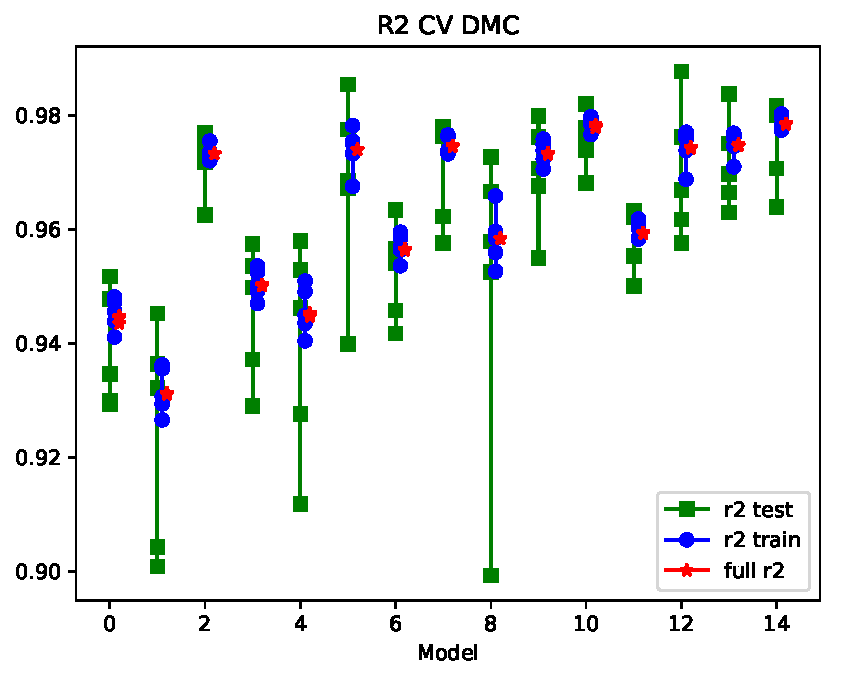
\includegraphics[width=1.0\textwidth]{../qwalk/ub3lyp_s1_/analysis/cv_valid.pdf}
\caption{5-fold CV regressions for model selection}
\end{figure}

%Figure 3
\begin{figure}
\centering
\begin{subfigure}{.5\textwidth}
  \centering
  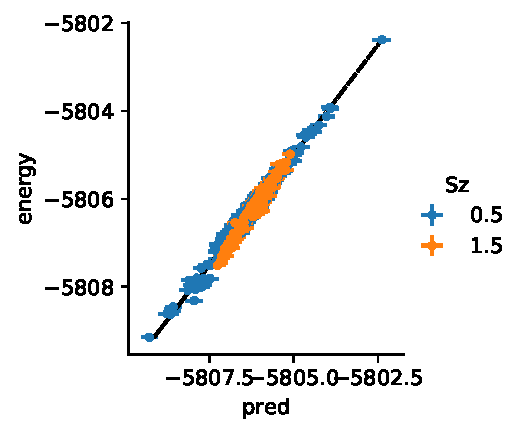
\includegraphics[width=\linewidth]{../qwalk/ub3lyp_s1_/analysis/fit.pdf}
  \caption{DMC predictions for all samples.}
  \label{fig:sub6}
\end{subfigure}%
\begin{subfigure}{.5\textwidth}
  \centering
  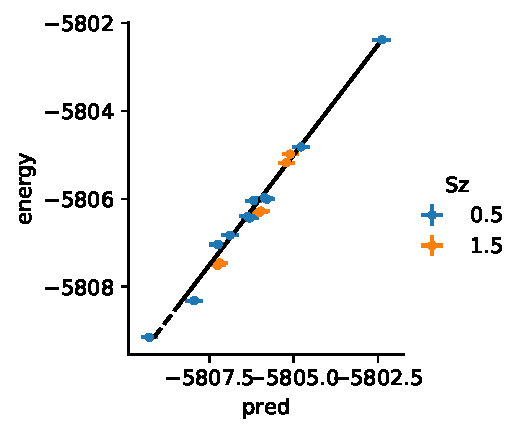
\includegraphics[width=\linewidth]{../qwalk/ub3lyp_s1_/analysis/fit_baseonly.pdf}
  \caption{DMC predictions for basestates. }
  \label{fig:sub7}
\end{subfigure}
\label{fig:test2}
\caption{DMC regression using all states and $\beta=2.0$.}
\end{figure}

%Figure 4
\begin{figure}
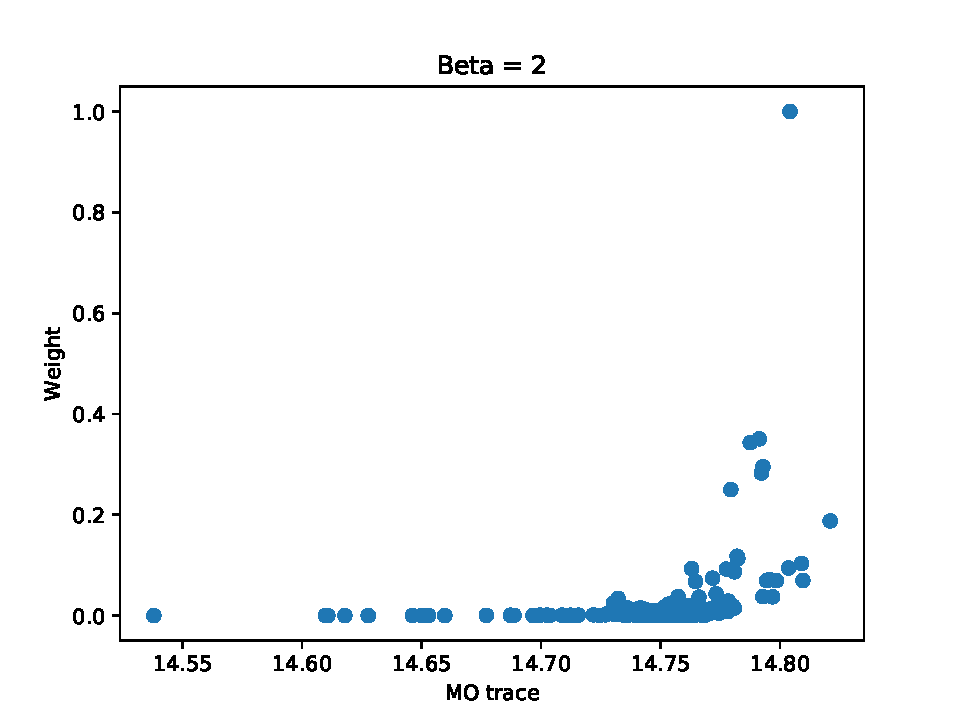
\includegraphics[width=1.0\textwidth]{../qwalk/ub3lyp_s1_/analysis/w_vs_t.pdf}
\caption{Weights versus trace for linear regression with $\beta=2.0$.}
\end{figure}

%Figure 5
\begin{figure}
\centering
\begin{subfigure}{.5\textwidth}
  \centering
  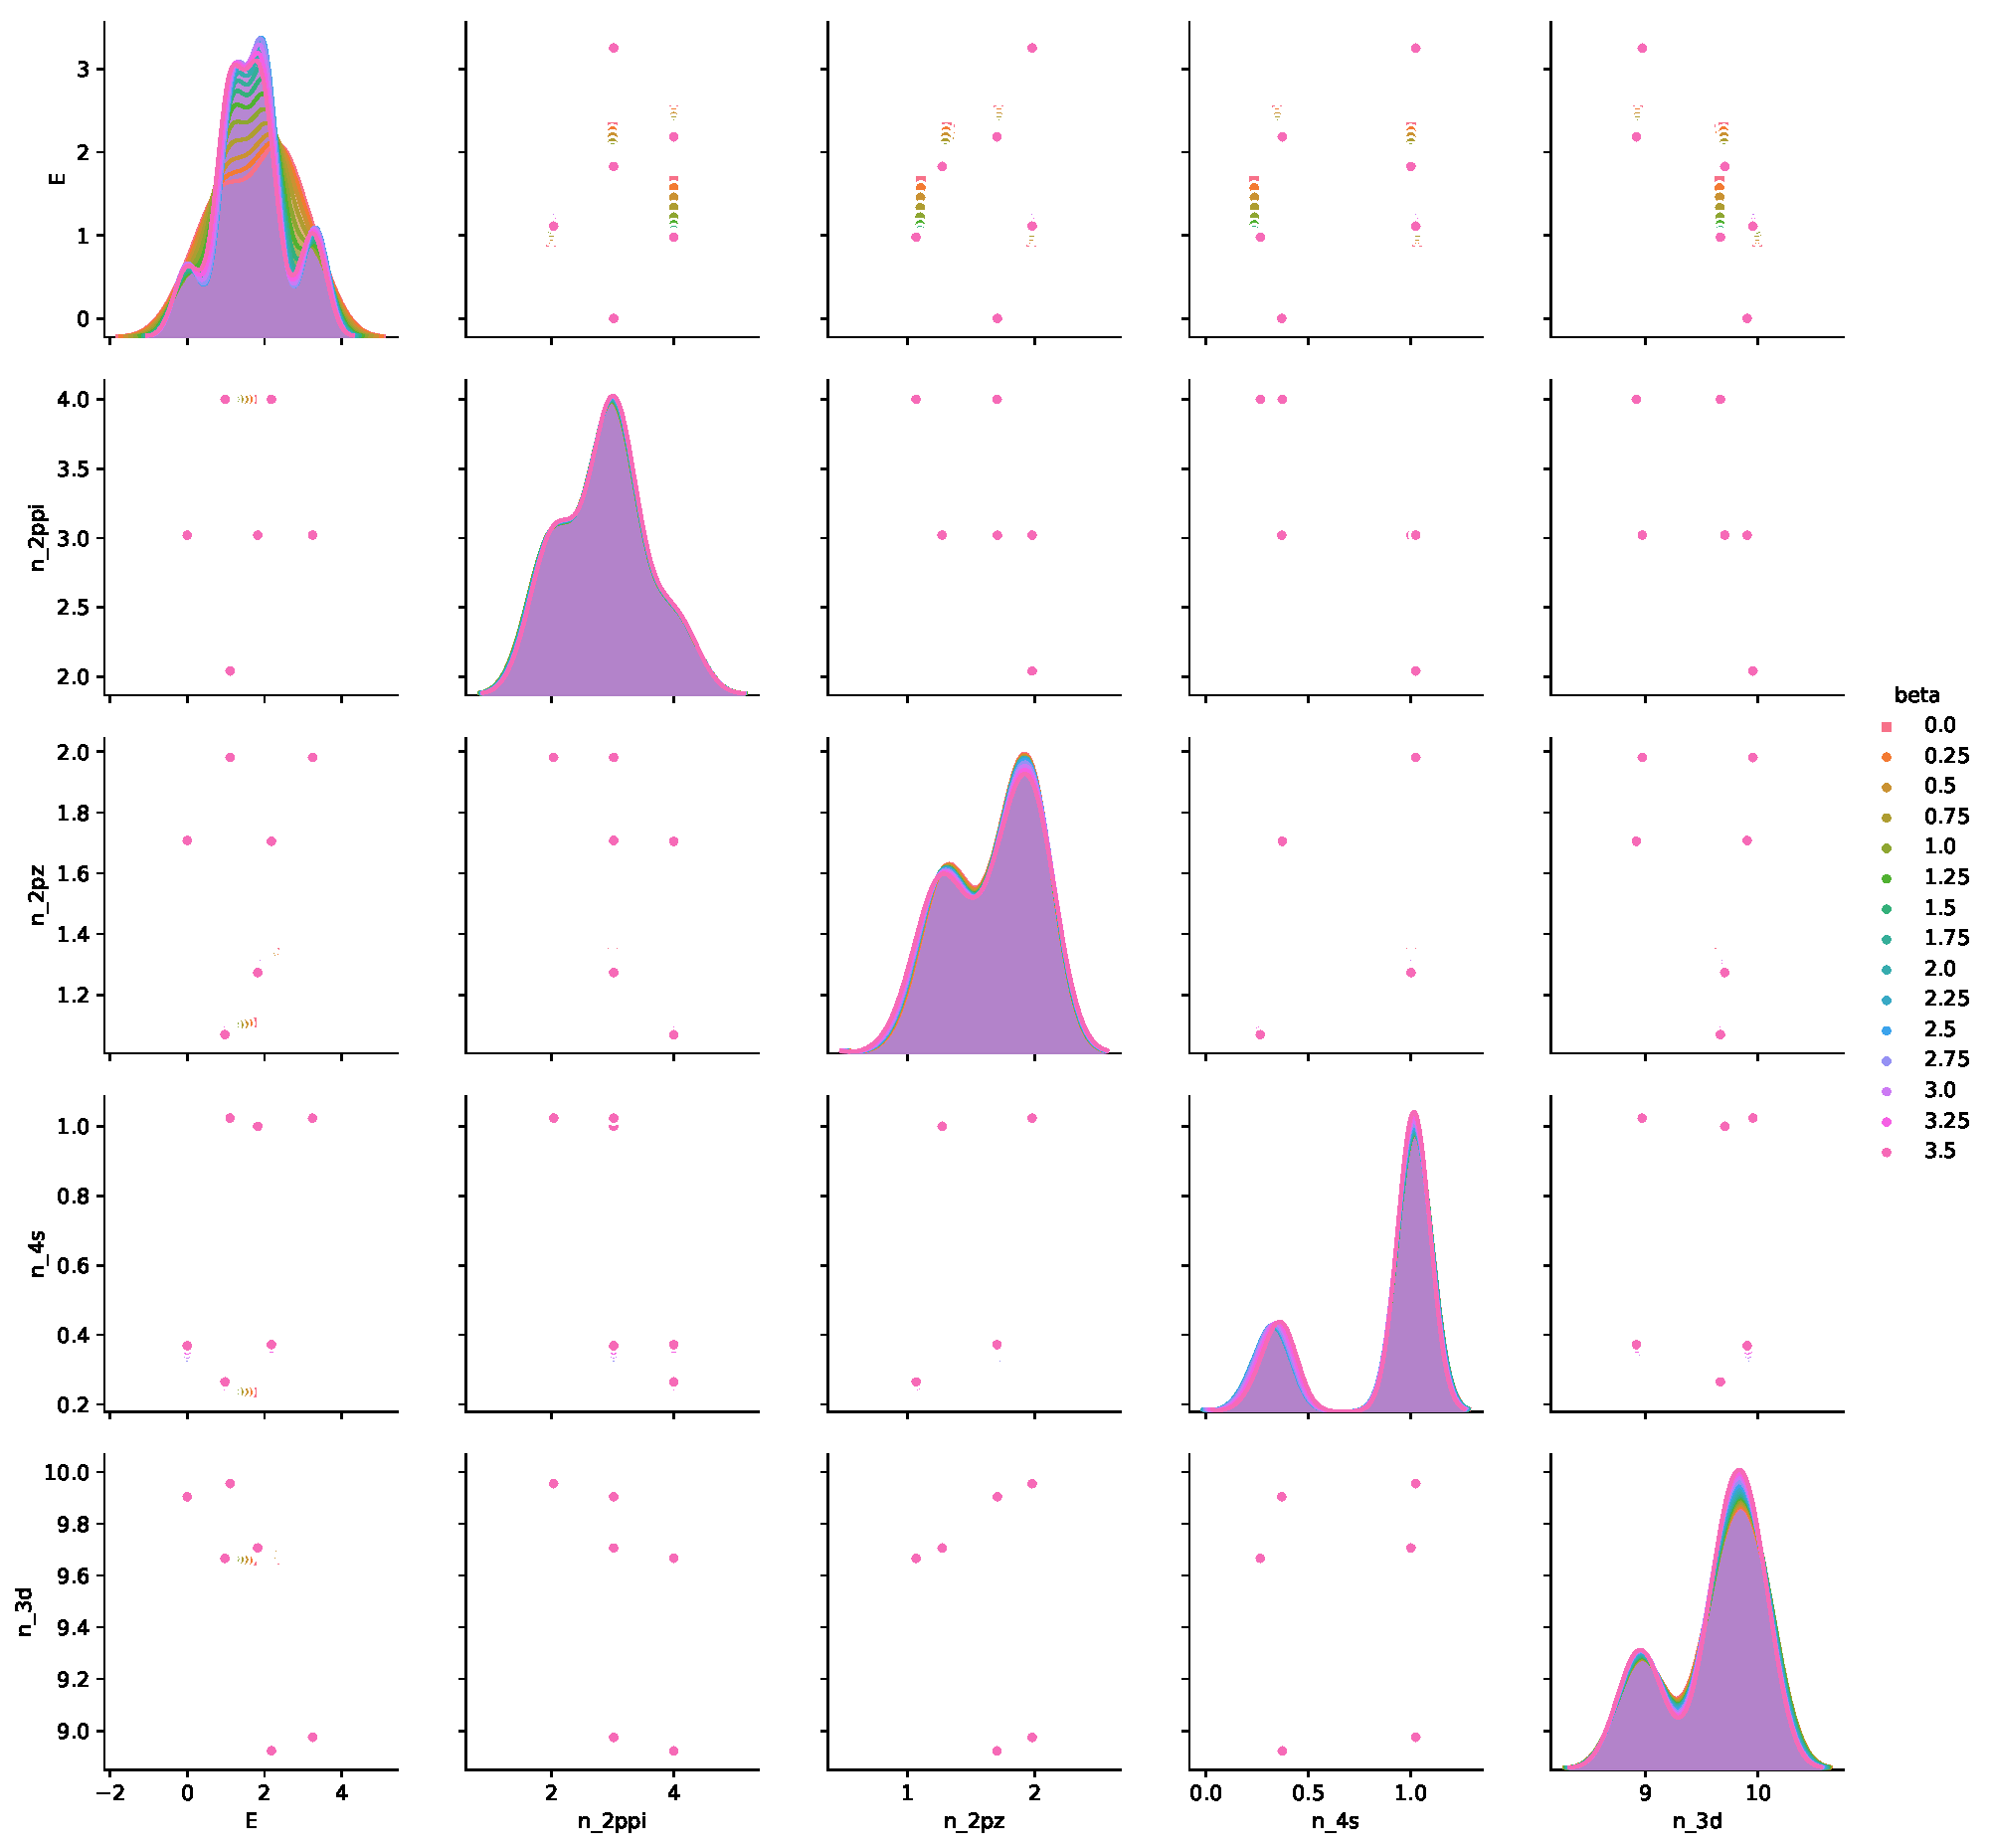
\includegraphics[width=\linewidth]{../qwalk/ub3lyp_s1_/analysis/beta_dmc_eigenvalues.pdf}
  \caption{Eigenvalues of DMC fit model, hue $\beta$.}
  \label{fig:sub1}
\end{subfigure}%
\begin{subfigure}{.5\textwidth}
  \centering
  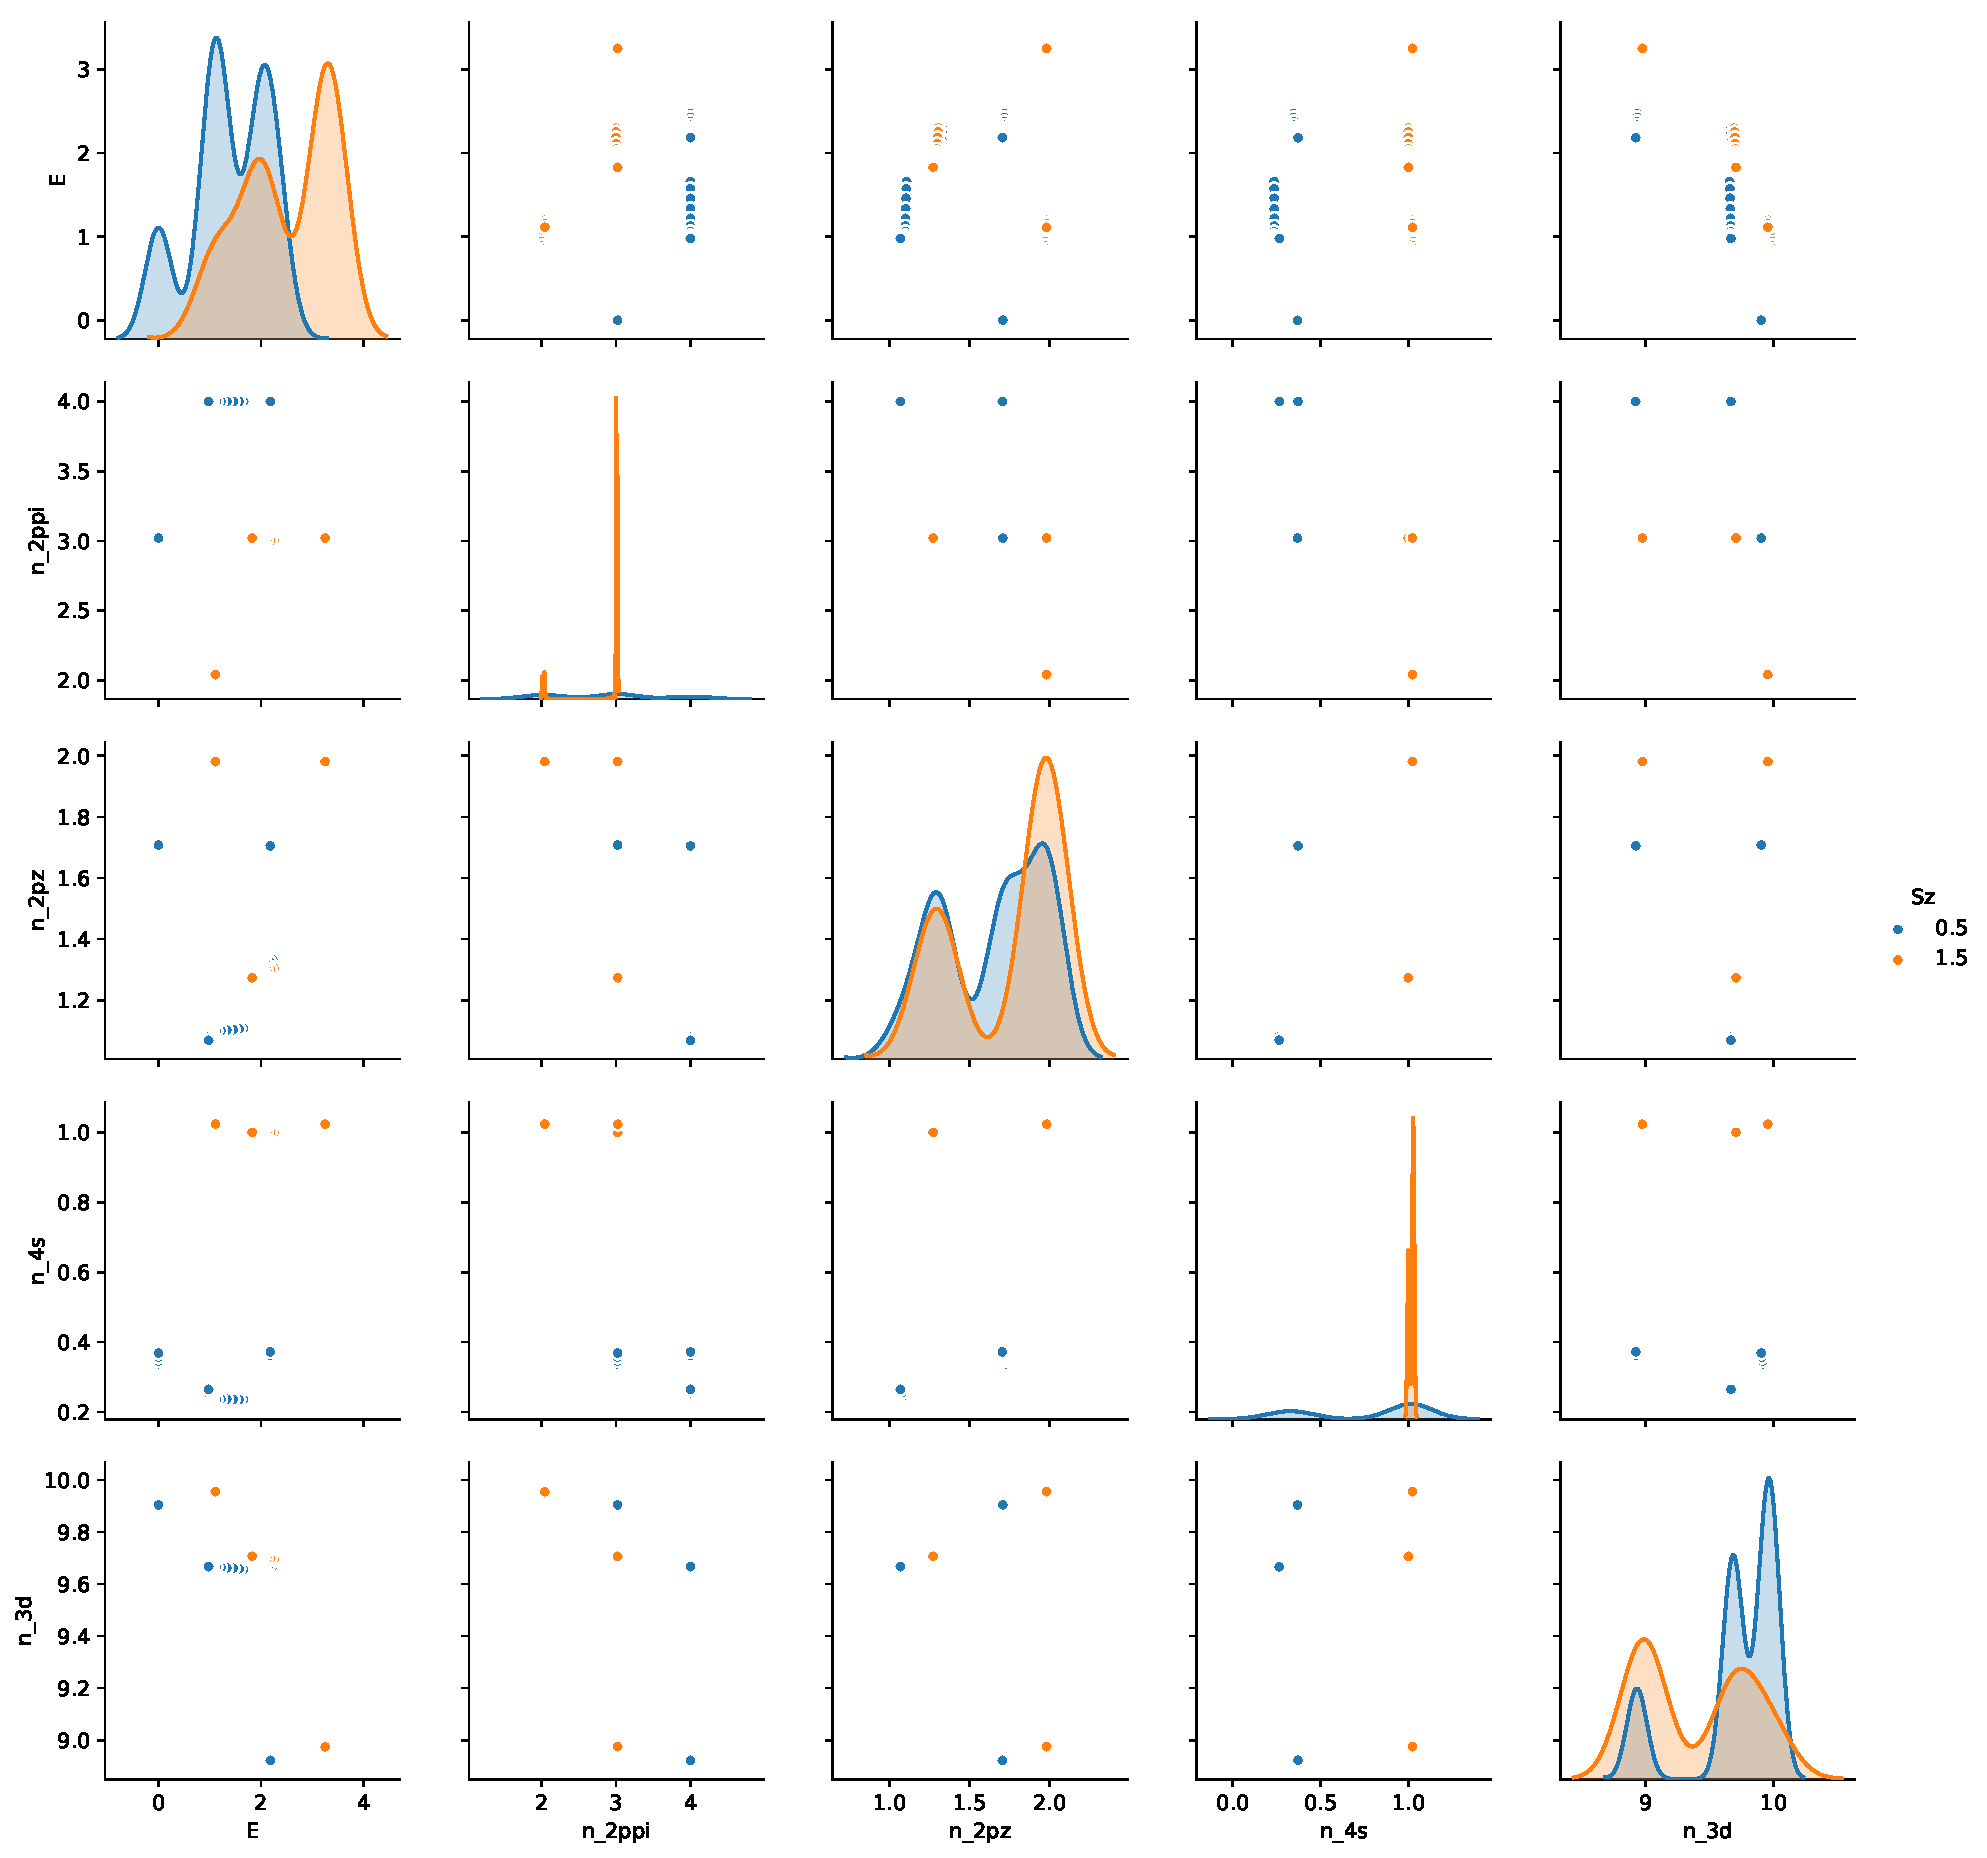
\includegraphics[width=\linewidth]{../qwalk/ub3lyp_s1_/analysis/beta_dmc_eigenvalues_sz.pdf}
  \caption{Eigenvalues of DMC fit model, hue $S_z$.}
  \label{fig:sub2}
\end{subfigure}
\label{fig:test1}
\caption{Eigenstates of models from DMC}
\end{figure}

%Figure 6
\begin{figure}
\centering
\begin{subfigure}{.5\textwidth}
  \centering
  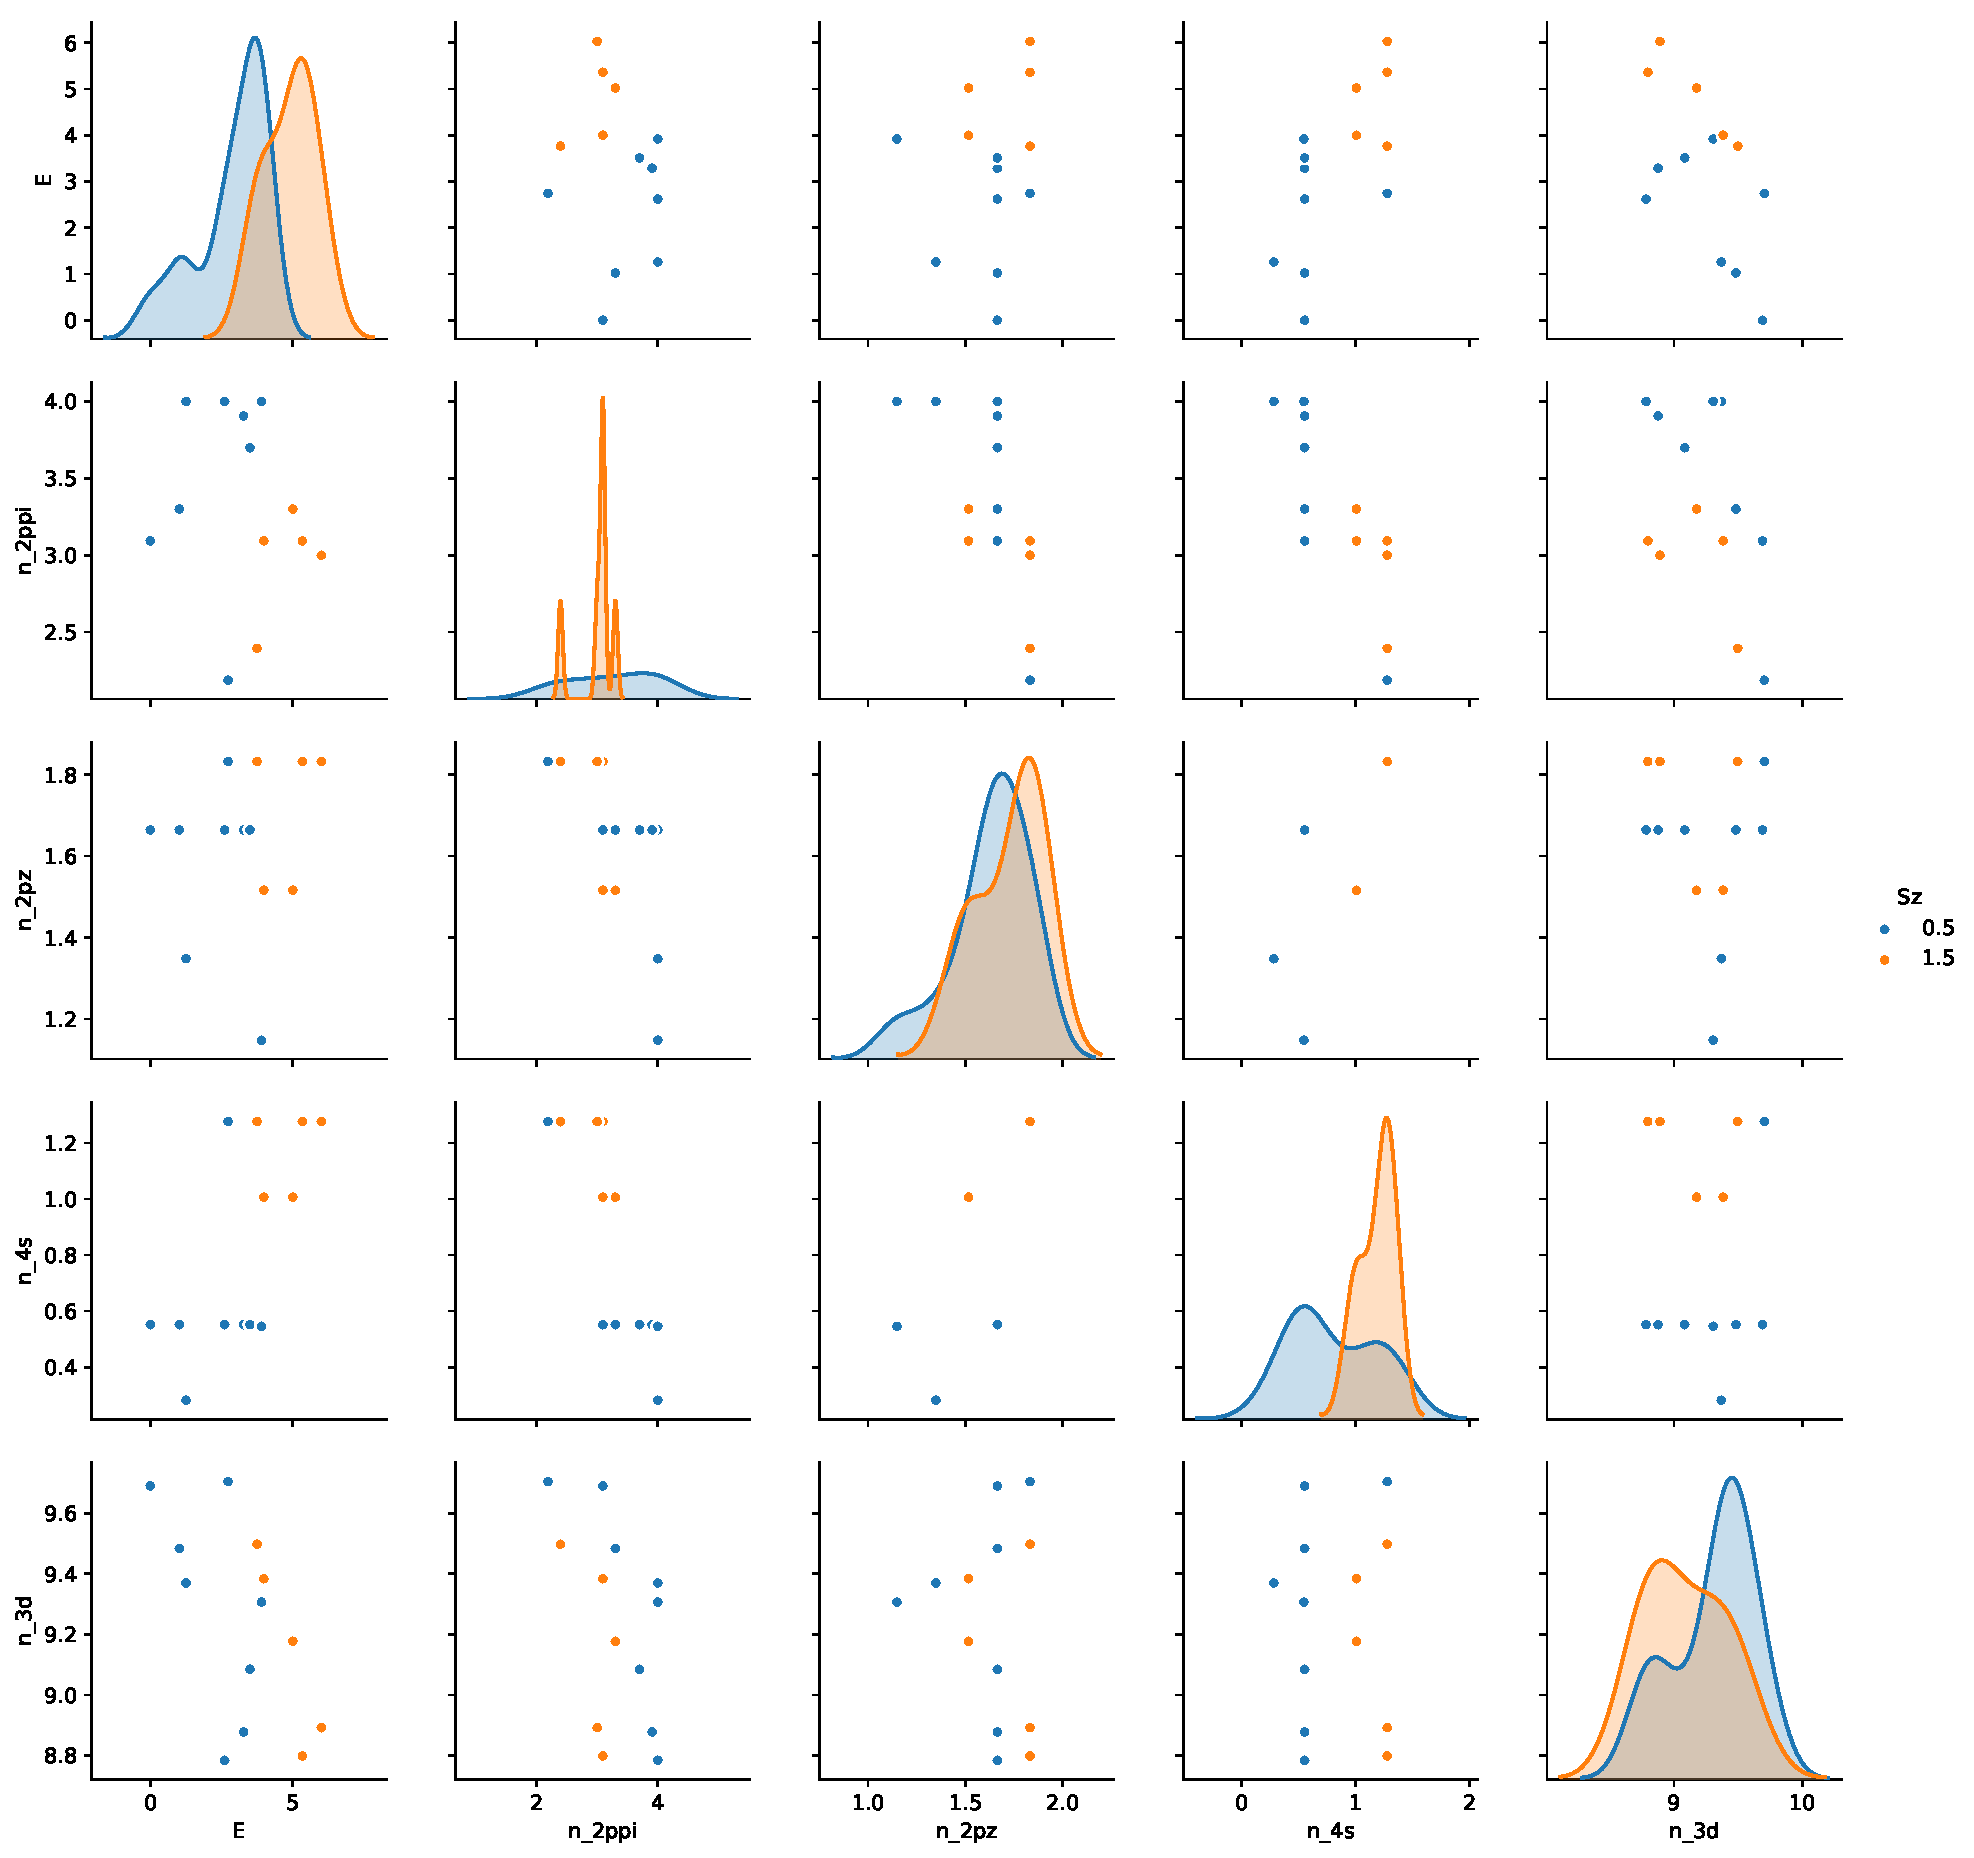
\includegraphics[width=\linewidth]{../qwalk/ub3lyp_s1_/analysis/roks_eigenvalues.pdf}
  \caption{Eigenvalues of ROKS effective model.}
  \label{fig:sub3}
\end{subfigure}%
\begin{subfigure}{.5\textwidth}
  \centering
  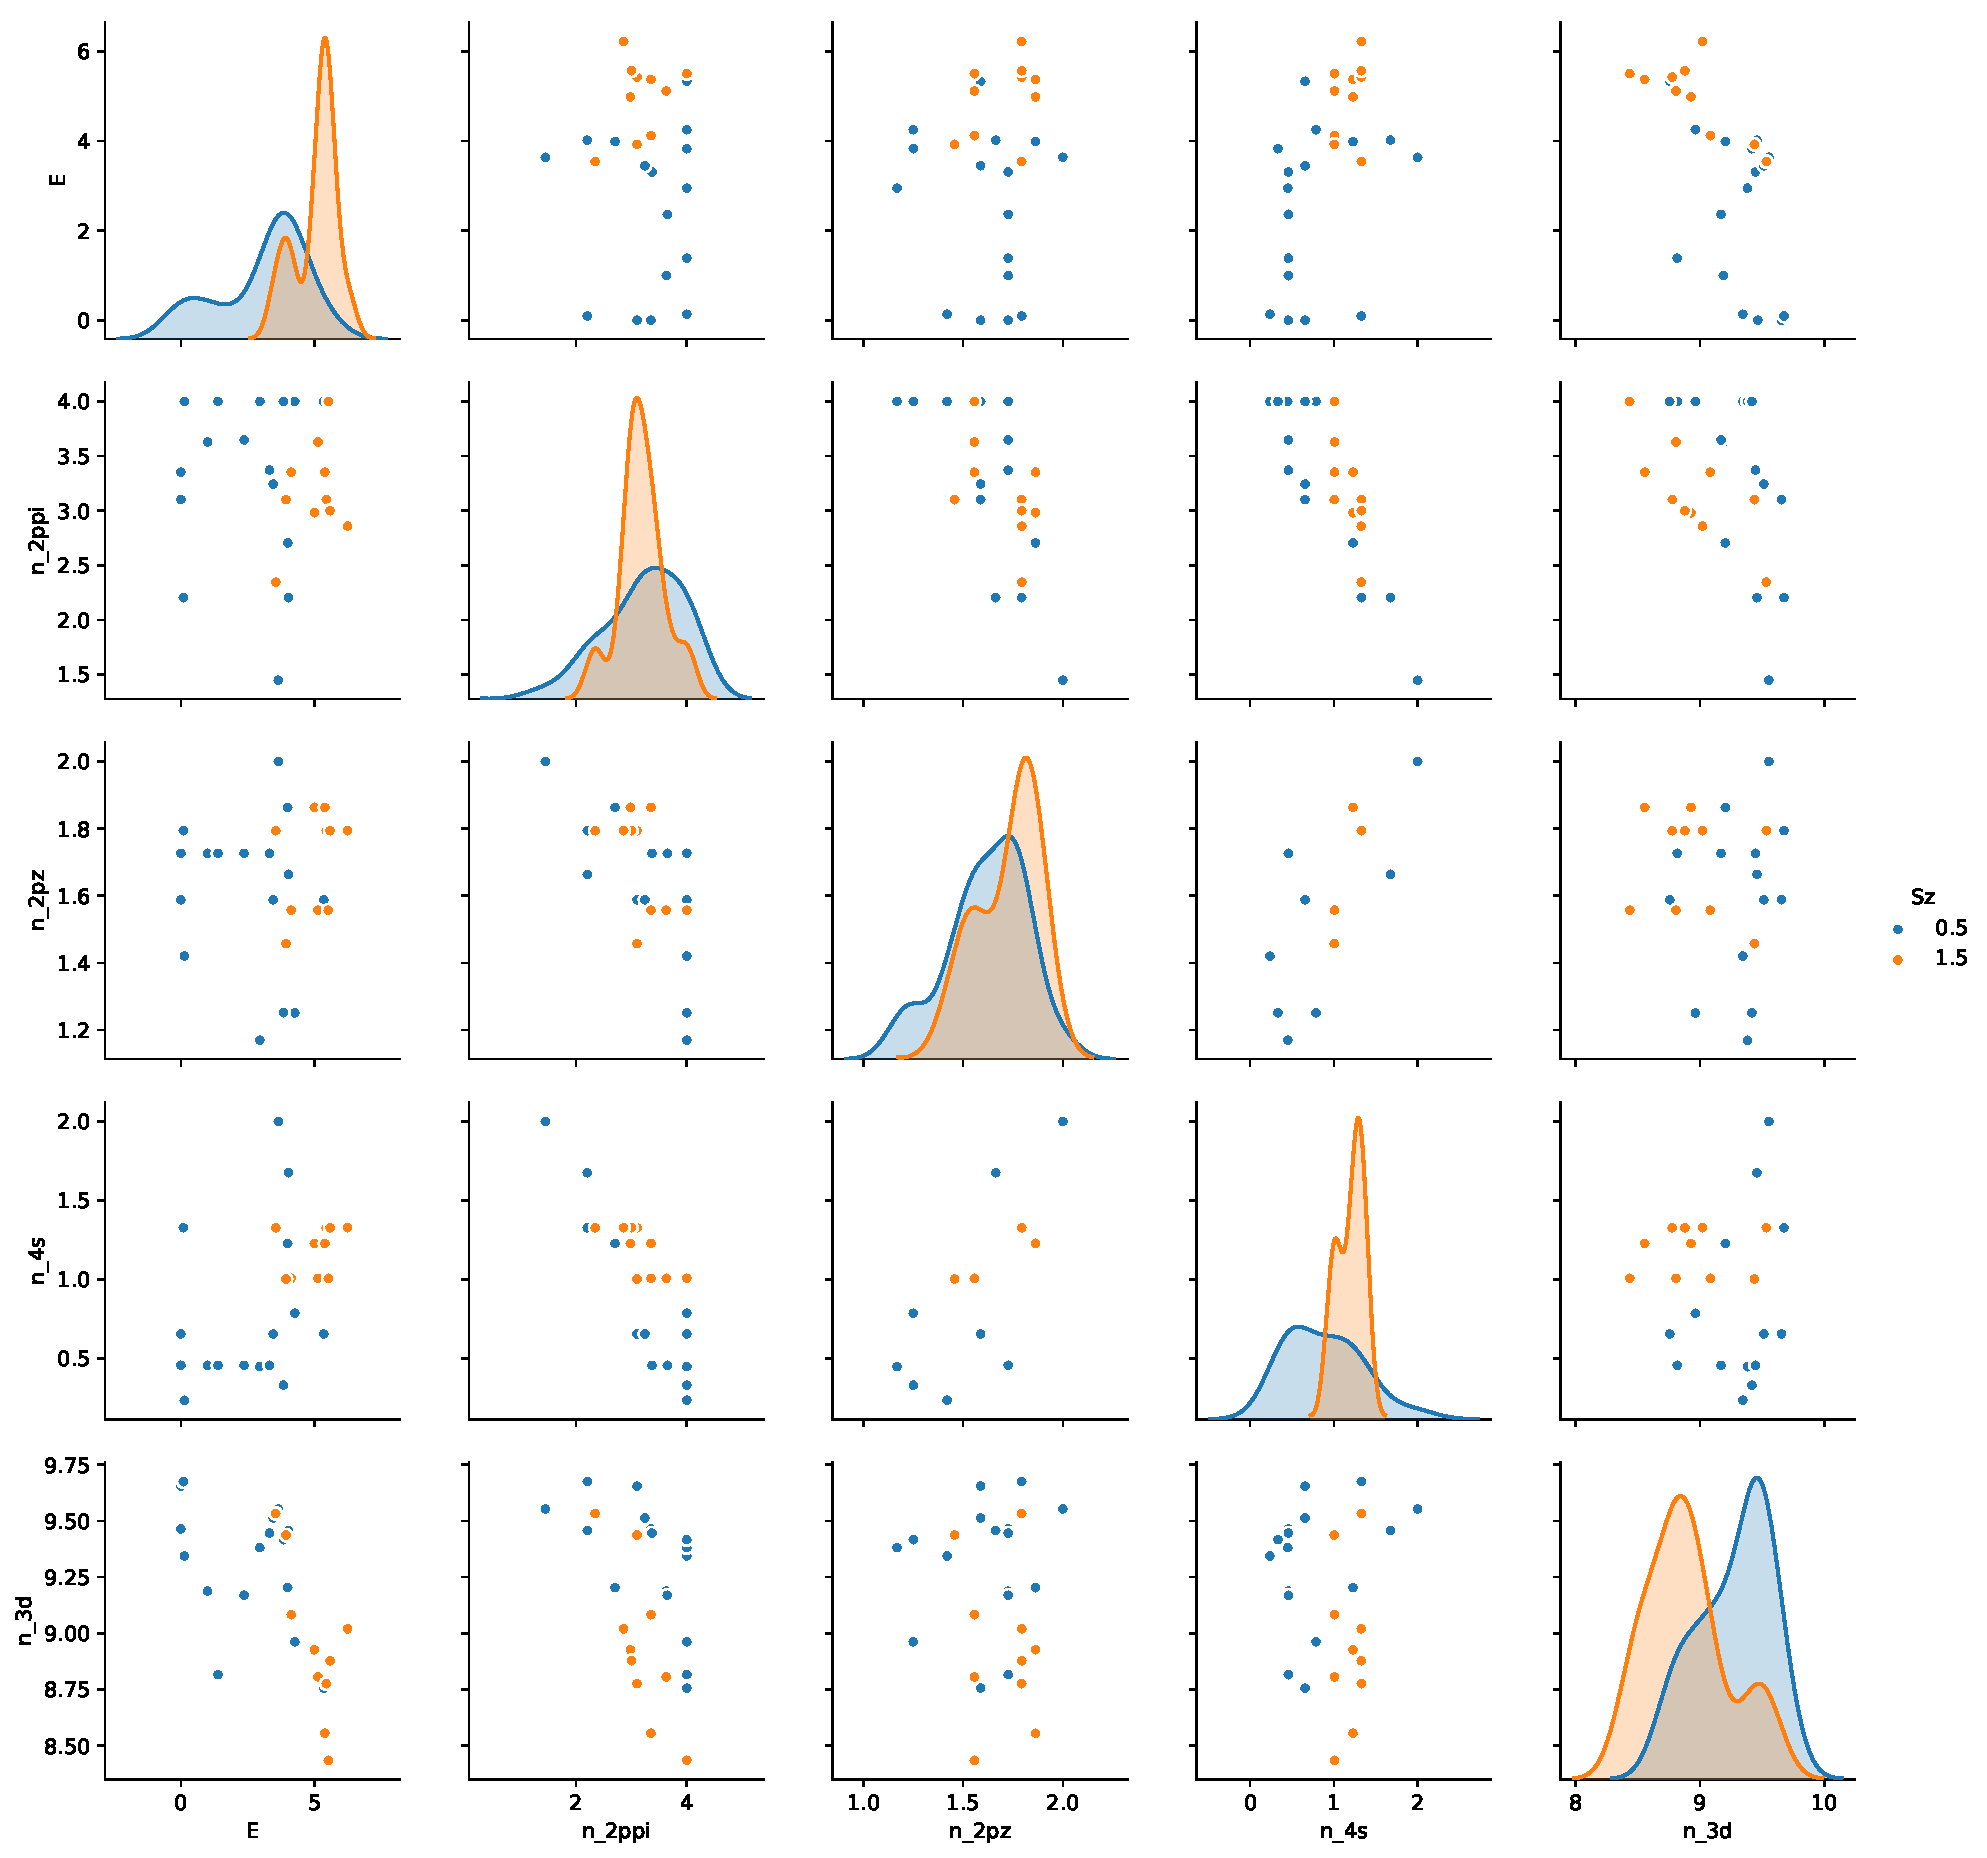
\includegraphics[width=\linewidth]{../qwalk/ub3lyp_s1_/analysis/uks_eigenvalues.pdf}
  \caption{Eigenvalues of UKS effective model.}
  \label{fig:sub4}
\end{subfigure}
\label{fig:test2}
\caption{Eigenstates of 1-particle models from DFT}
\end{figure}

%Table
%\begin{wrapfigure}{r}{0.4\textwidth}
%\begin{tabular}{lll}
% &  DMC (eV) & ROKS (eV) \\
%$\epsilon_{d_\delta}$ &  0.00 & 0.00  \\
%$\epsilon_{d_\pi}$ & -0.10 & -0.36 \\
%$\epsilon_{d_{z^2}}$ & 0.41 & 0.52 \\
%$\epsilon_z$ & 1.20 & 0.66 \\
%$\epsilon_\pi$ & 2.21 & 0.85 \\
%$\epsilon_s$ &  2.44 & 4.24 \\
%$t_\pi$ & -0.22 & -1.14 \\
%$t_{s d_{z^2}}$ & 0.38 & 0.97 \\
%$t_{s z}$ & 0.80 & 1.86\\
%$t_{d_{z^2} z}$ & 0.70 & 1.55\\
%$J_{sd}$ & -0.51 & 0.00 \\ 
%$U_s$ & 3.91 & 0.00 \\
%\end{tabular}
%\caption{Parameter differences between DFT/DMC models}
%\end{wrapfigure}
\end{document}